\section{Simulation Results}%
\label{sec:simulations}

\begin{figure}[t]
    \centerline{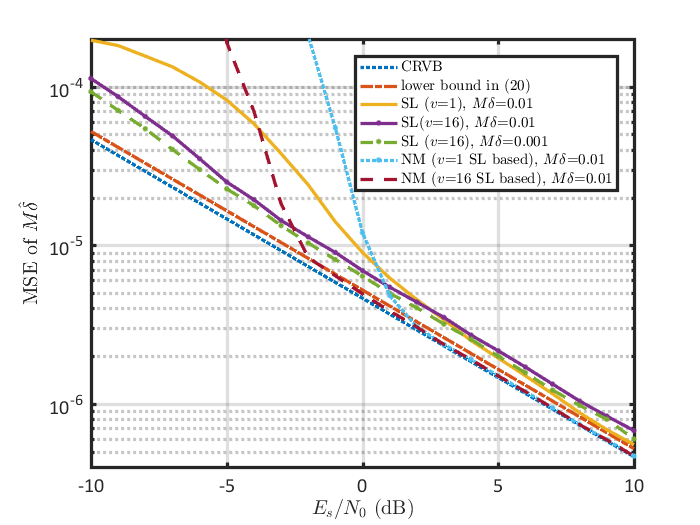
\includegraphics[width=3.25in]{accuracy_NM_SL.png}}
    \caption{Accuracy of the NM and the SL estimators ($L_0=32$, $M=2$)}
    \label{fig:accuracy_NM_SL}
    \end{figure}

\begin{figure}[t]
    \centerline{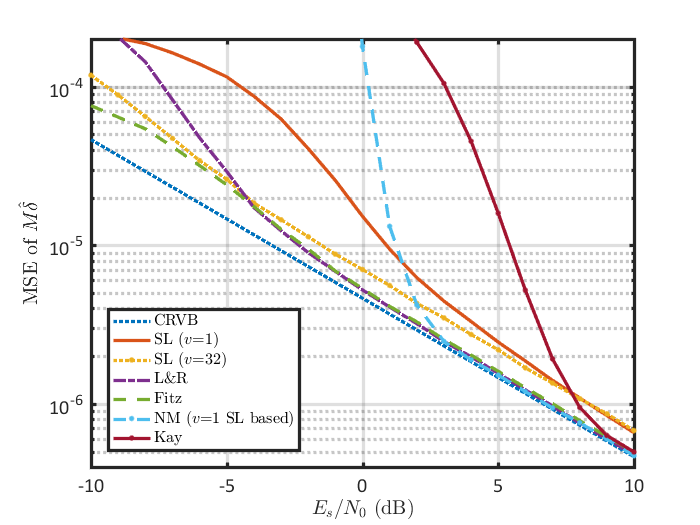
\includegraphics[width=3.25in]{accuracy_NM_SL_traditional.png}}
    \caption{Accuracy of the SL, the NM and the traditional estimators ($L_0=32$, $M=2$, $M\delta=0.01$)}
    \label{fig:accuracy_NM_SL_traditional}
    \end{figure}

\begin{figure}[t]
    \centerline{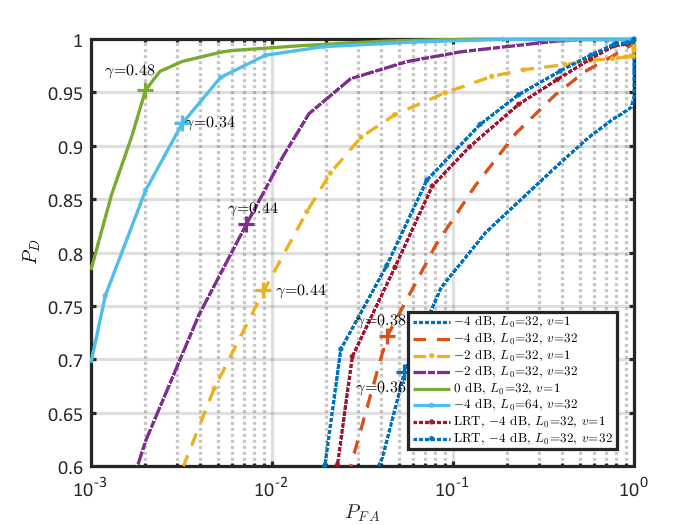
\includegraphics[width=3.25in]{ROC_new.png}}
    \caption{Receiver operating characteristics (ROC) of the sequential detector ($M=2$, $M\delta=0.01$)}
    \label{fig:Receiver operating characteristics}
    \end{figure}

In the simulation section, we reverse the order of discussion by first showing 
the accuracy of estimators in carrier synchronization and then showing some results of sequential detection since
the GLRT based detector in~\eqref{eq:generalized_corr} relies on the accuracy of 
the SL estimator. The symbol sequence of the preamble is chosen as a Gold sequence 
with good autocorrelation property and
modulated by a QPSK alphabet.
The pulse is chosen a 0.5
rolloff Square-Root Raised Cosine (SRRC) pulse to satisfy the (squared root of) Nyquist property.
The normalized frequency offset $\delta$ is intentionally set to be in the safe estimation range for all estimators for simulation purpose.

\subsection{Simulation Results for Estimation}

% \begin{figure}[t]
%     \centerline{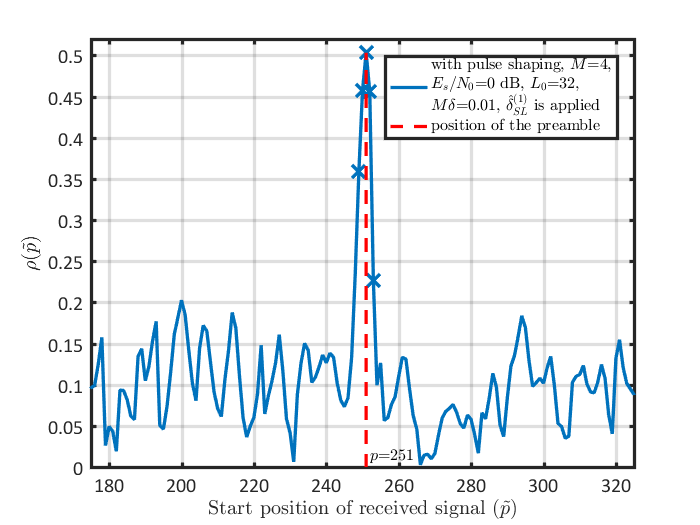
\includegraphics[width=3.4in]{generalized_correlation_p_plus_delta.png}}
%     \caption{Performance of sequential detector when the preamble is pulse shaped}
%     \label{fig:Generalized correlation}
%     \end{figure}

Figure~\ref{fig:accuracy_NM_SL} illustrates the accuracy of single-lag (SL) and the NM estimator.
Compared with the two curves of SLs with $v{=}1$ and $v{=}32$, 
we see the length-$32$ partial correlating
improves the accuracy of SL by providing an approximate $4$ dB relative processing gain at negative SNRs (near $\text{SNR}=-5$ dB).
More-over, we see the SL with $v=1$ starts to have a better accuracy 
at 10 dB SNR than the SL with $v=32$. The gap is due to the Dirichlet function with
respect to $v|\delta|$ increases the variance and going to be increased as 
SNR increases.
For the same reason, the accuracy of SL with $v=32$ at small frequency offset has a better accuracy at all SNRs.

The SL estimators don't approach the CRVB~\cite{Gini_98} while the NM does. 
We also see the NM estimator achieves a good acc-uracy 
based on the starting point of SL with $v=32$ at lower SNR
because the latter provides enough accuracy. 
In contrast, the NM estimator based on SL with $v=1$ has worse accuracy than SL 
at all negative SNRs because the accuracy of SL is not enough so that the Newton iteration converges occasionally to 
other local minimum away from the true frequency offset.

Figure~\ref{fig:accuracy_NM_SL_traditional} compares the accuracy of our proposed estimators
and traditional estimators in~\cite{kay_89,Fitz_94,Luise_Reggiannini_95}. It shows when 
frequency offset is small, our NM estimator has a slightly better accuracy than traditional estimators at moderate SNRs.
The drawback of the NM estimator is the poor accuracy at low SNRs since it depends on the 
SL. Thus, a family of the SL with $v=32$ and the NM based on the SL with $v=1$ can be used 
to achieve a good accuracy at most SNRs.

\subsection{Simulation Results for Detection}

% Figure~\ref{fig:Generalized correlation} shows the performance of sequential detector
% in~\eqref{eq:generalized_corr} at each received signal windows. Note, because of pulse sha-ping,
% the autocorrelation property of the preamble sequence is decreased, which results
% the correlations at adjacent windows near the position of the preamble decay slow and thus make much challenges
% to choose threshold to make correct dicision.

% The solution is to adjust the detection algorithm by finding the local maximum of the correlation
% instead of just comparing the correlation with the threshold at each window. Note, when count for the ratio of false alarm and detection (for determining the threshold),
% the two positions should be counted as latter.

Figure~\ref{fig:Receiver operating characteristics} shows the receiver operating characteristics (ROC) of the detection algorithm.
The better accuracy of SL with par-tial correlating at low SNRs also increases the performance of detection, e.g.,
at $-2$ dB SNR, $\gamma=0.44$, the false alarm probability $P_{FA}$ of SL with $v=32$ is reduced $0.2\%$ and 
the detection probability $P_{D}$ is $5\%$ larger compared with the SL with $v{=}1$.
The figure also shows the detector doesn't work well at $-4$ dB SNR if only $32$ symbols of preamble are used;  
The performance is significantly improved by doubling the number of symbols.
